\documentclass[UTF8,11pt]{ctexart}
\usepackage[a4paper,margin=22mm]{geometry}
\usepackage{graphicx,enumitem,amssymb,tabularx}
\usepackage[normalem]{ulem}
\usepackage{xeCJKfntef}
\setlength{\parindent}{0pt}
\setlength{\parskip}{.6em}
\sloppy
\begin{document}
\section*{2012年考研英语二}
2012 年全国硕士研究生招生考试英语（二）


\subsection*{\textbf{Section I Use of English}}


\subsection*{\textbf{Directions:}}


Read the following text. Choose the best word(s) for each numbered blank and mark A, B, C or D on the ANSWER SHEET. (10 points)


Millions of Americans and foreigners see G.I. Joe as a mindless war toy, the symbol of American military adventurism, but that’s not how it used to be. To the men and women who \uline{1} in World War II and the people they liberated, the G.I. was the \uline{2} man grown into hero, the poor farm kid torn away from his home, the guy who \uline{3} all the burdens of battle, who slept in cold foxholes, who went without the \uline{4} of food and shelter, who stuck it out and drove back the Nazi reign of murder. This was not a volunteer soldier, not someone well paid, \uline{5} an average guy, up \uline{6} the best trained, best equipped, fiercest, most brutal enemies seen in centuries.


His name isn’t much. G.I. is just a military abbreviation \uline{7} Government Issue, and it was on all of the articles \uline{8} to soldiers. And Joe? A common name for a guy who never \uline{9} it to the top. Joe Blow, Joe Palooka, Joe Magrac… a working class name. The United States has \uline{10} had a president or vice-president or secretary of state Joe.


G.I. Joe had a \uline{11} career fighting German, Japanese, and Korean troops. He


appears as a character, or a \uline{12} of American personalities, in the 1945 movie \textit{The} \textit{Story of G.I. Joe}, based on the last days of war correspondent Ernie Pyle. Some of the soldiers Pyle \uline{13} portrayed themselves in the film. Pyle was famous for covering the \uline{14} side of the war, writing about the dirt-snow-and-mud soldiers, not how many miles were \uline{15} or what towns were captured or liberated. His reports \uline{16} the “Willie” cartoons of famed \textit{Stars and Stripes} artist Bill Maulden. Both men \uline{17} the dirt and exhaustion of war, the \uline{18} of civilization that the soldiers shared with each other and the civilians: coffee, tobacco, whiskey, shelter, sleep. \uline{19} Egypt, France, and a dozen more countries, G.I. Joe was any American soldier, \uline{20} the most important person in their lives.


\noindent\begin{tabularx}{\linewidth}{@{}lXXXX@{}}1. & \textbf{A.} served & \textbf{B.} performed & \textbf{C.} rebelled & \textbf{D.} betrayed\\\end{tabularx}\par

\noindent\begin{tabularx}{\linewidth}{@{}lXXXX@{}}2. & \textbf{A.} actual & \textbf{B.} common & \textbf{C.} special & \textbf{D.} normal\\\end{tabularx}\par

\noindent\begin{tabularx}{\linewidth}{@{}lXXXX@{}}3. & \textbf{A.} loaded & \textbf{B.} eased & \textbf{C.} removed & \textbf{D.} bore\\\end{tabularx}\par

\noindent\begin{tabularx}{\linewidth}{@{}lXXXX@{}}4. & \textbf{A.} necessities & \textbf{B.} facilities & \textbf{C.} commodities & \textbf{D.} properties\\\end{tabularx}\par

\noindent\begin{tabularx}{\linewidth}{@{}lXXXX@{}}5. & \textbf{A.} and & \textbf{B.} nor & \textbf{C.} but & \textbf{D.} hence\\\end{tabularx}\par

\noindent\begin{tabularx}{\linewidth}{@{}lXXXX@{}}6. & \textbf{A.} for & \textbf{B.} into & \textbf{C.} from & \textbf{D.} against\\\end{tabularx}\par

\noindent\begin{tabularx}{\linewidth}{@{}lXXXX@{}}7. & \textbf{A.} implying & \textbf{B.} meaning & \textbf{C.} symbolizing & \textbf{D.} claiming\\\end{tabularx}\par

\noindent\begin{tabularx}{\linewidth}{@{}lXXXX@{}}8. & \textbf{A.} handed out & \textbf{B.} turned over & \textbf{C.} brought back & \textbf{D.} passed down\\\end{tabularx}\par

\noindent\begin{tabularx}{\linewidth}{@{}lXXXX@{}}9. & \textbf{A.} pushed & \textbf{B.} got & \textbf{C.} made & \textbf{D.} managed\\\end{tabularx}\par

\noindent\begin{tabularx}{\linewidth}{@{}lXXXX@{}}10. & \textbf{A.} ever & \textbf{B.} never & \textbf{C.} either & \textbf{D.} neither\\\end{tabularx}\par

\noindent\begin{tabularx}{\linewidth}{@{}lXXXX@{}}11. & \textbf{A.} disguised & \textbf{B.} disturbed & \textbf{C.} disputed & \textbf{D.} distinguished\\\end{tabularx}\par

\noindent\begin{tabularx}{\linewidth}{@{}lXXXX@{}}12. & \textbf{A.} company & \textbf{B.} community & \textbf{C.} collection & \textbf{D.} colony\\\end{tabularx}\par

\noindent\begin{tabularx}{\linewidth}{@{}lXXXX@{}}13. & \textbf{A.} employed & \textbf{B.} appointed & \textbf{C.} interviewed & \textbf{D.} questioned\\\end{tabularx}\par

\noindent\begin{tabularx}{\linewidth}{@{}lXXXX@{}}14. & \textbf{A.} human & \textbf{B.} military & \textbf{C.} political & \textbf{D.} ethical\\\end{tabularx}\par

\noindent\begin{tabularx}{\linewidth}{@{}lXXXX@{}}15. & \textbf{A.} ruined & \textbf{B.} commuted & \textbf{C.} patrolled & \textbf{D.} gained\\\end{tabularx}\par

\noindent\begin{tabularx}{\linewidth}{@{}lXXXX@{}}16. & \textbf{A.} paralleled & \textbf{B.} counteracted & \textbf{C.} duplicated & \textbf{D.} contradicted\\\end{tabularx}\par

\noindent\begin{tabularx}{\linewidth}{@{}lXXXX@{}}17. & \textbf{A.} neglected & \textbf{B.} emphasized & \textbf{C.} avoided & \textbf{D.} admired\\\end{tabularx}\par

\noindent\begin{tabularx}{\linewidth}{@{}lXXXX@{}}18. & \textbf{A.} stages & \textbf{B.} illusions & \textbf{C.} fragments & \textbf{D.} advances\\\end{tabularx}\par

\noindent\begin{tabularx}{\linewidth}{@{}lXXXX@{}}19. & \textbf{A.} With & \textbf{B.} To & \textbf{C.} Among & \textbf{D.} Beyond\\\end{tabularx}\par

\noindent\begin{tabularx}{\linewidth}{@{}lXXXX@{}}20. & \textbf{A.} on the contrary & \textbf{B.} by this means & \textbf{C.} from the outset & \textbf{D.} at that point\\\end{tabularx}\par

\subsection*{\textbf{Section II Reading Comprehension}}


\subsection*{\textbf{Part A}}


\subsection*{\textbf{Directions:}}


Read the following four texts. Answer the questions after each text by choosing A, B, C or D. Mark your answers on the ANSWER SHEET. (40 points)


\subsection*{\textbf{Text 1}}


Homework has never been terribly popular with students and even many parents, but in recent years it has been particularly scorned. School districts across the country, most recently Los Angeles Unified, are revising their thinking on this educational ritual. Unfortunately, L.A. Unified has produced an inflexible policy which mandates that with the exception of some advanced courses, homework may no longer count for more than 10\% of a student’s academic grade.


This rule is meant to address the difficulty that students from impoverished or chaotic homes might have in completing their homework. But the policy is unclear and contradictory. Certainly, no homework should be assigned that students cannot complete on their own or that they cannot do without expensive equipment. But if the district is essentially giving a pass to students who do not do their homework because of complicated family lives, it is going riskily close to the implication that standards need to be lowered for poor children.


District administrators say that homework will still be a part of schooling; teachers are allowed to assign as much of it as they want. But with homework counting for no more than 10\% of their grades, students can easily skip half their homework and see very little difference on their report cards. Some students might do well on state tests without completing their homework, but what about the students who performed well on the tests and did their homework? It is quite possible that the homework helped. Yet rather than empowering teachers to find what works best for their students, the policy imposes a flat, across-the-board rule.


At the same time, the policy addresses none of the truly thorny questions about homework. If the district finds homework to be unimportant to its students’ academic achievement, it should move to reduce or eliminate the assignments, not make them count for almost nothing. Conversely, if homework matters, it should account for a significant portion of the grade. Meanwhile, this policy does nothing to ensure that the homework students receive is meaningful or appropriate to their age and the subject, or that teachers are not assigning more than they’re willing to review and correct.


The homework rules should be put on hold while the school board, which is responsible for setting educational policy, looks into the matter and conducts public hearings. It is not too late for L.A. Unified to do homework right.


21. It is implied in Paragraph 1 that nowadays homework \_\_\_\_


\begin{itemize}[leftmargin=2em,itemsep=.2em,topsep=.4em]\item[A.] is receiving more criticism.
\item[B.] is gaining more preferences.
\item[C.] is no longer an educational ritual.
\item[D.] is not required for advanced courses.
\end{itemize}

22.


\begin{itemize}[leftmargin=2em,itemsep=.2em,topsep=.4em]\item[A.] tend to have moderate expectations for their education.
\item[B.] have asked for a different educational standard.
\item[C.] may have problems finishing their homework.
\item[D.] have voiced their complaints about homework.
\item[L.] A. Unified has made the rule about homework mainly because poor students \_\_\_\_
\end{itemize}

23. According to Paragraph 3, one problem with the policy is that it may \_\_\_\_


\begin{itemize}[leftmargin=2em,itemsep=.2em,topsep=.4em]\item[A.] result in students’ indifference to their report cards.
\item[B.] undermine the authority of state tests.
\item[C.] restrict teachers’ power in education.
\item[D.] discourage students from doing homework.
\end{itemize}

24. As mentioned in Paragraph 4, a key question unanswered about homework is whether \_\_\_\_


\begin{itemize}[leftmargin=2em,itemsep=.2em,topsep=.4em]\item[A.] it should be eliminated.
\item[B.] it counts much in schooling.
\item[C.] it places extra burdens on teachers.
\item[D.] it is important for grades.
\end{itemize}

25. A suitable title for this text could be \_\_\_\_


\begin{itemize}[leftmargin=2em,itemsep=.2em,topsep=.4em]\item[A.] A Faulty Approach to Homework.
\item[B.] A Welcomed Policy for Poor Students.
\item[C.] Thorny Questions about Homework.
\item[D.] Wrong Interpretations of an Educational Policy.
\end{itemize}

\subsection*{\textbf{Text 2}}


Pretty in pink: adult women do not remember being so obsessed with the colour, yet it is pervasive in our young girls’ lives. It is not that pink is intrinsically bad, but \uline{it is} \uline{such a tiny slice of the rainbow }and, though it may celebrate girlhood in one way, it also repeatedly and firmly fuses girls’ identity to appearance. Then it presents that connection, even among two-year-olds, between girls as not only innocent but as evidence of innocence. Looking around, I despaired at the singular lack of imagination about girls’ lives and interests.


Girls’ attraction to pink may seem unavoidable, somehow encoded in their DNA, but according to Jo Paoletti, an associate professor of American Studies, it is not. Children were not colour-coded at all until the early 20th century: in the era before domestic washing machines all babies wore white as a practical matter, since the only way of getting clothes clean was to boil them. What’s more, both boys and girls wore what were thought of as gender-neutral dresses. When nursery colours were introduced, pink was actually considered the more masculine colour, a pastel version of red, which was associated with strength. Blue, with its intimations of the Virgin Mary, constancy and faithfulness, symbolised femininity. It was not until the mid-1980s, when amplifying age and sex differences became a dominant children’s marketing strategy, that pink fully came into its own, when it began to seem inherently attractive to girls, part of what defined them as female, at least for the first few critical years.


I had not realized how profoundly marketing trends dictated our perception of what is natural to kids, including our core beliefs about their psychological development. Take the toddler. I assumed that phase was something experts developed after years of research into children’s behaviour: wrong. Turns out, according to Daniel Cook, a historian of childhood consumerism, it was popularised as a marketing trick by clothing manufacturers in the 1930s.


Trade publications counselled department stores that, in order to increase sales, they should create a “third stepping stone” between infant wear and older kids’ clothes. It was only after “toddler” became a common shoppers’ term that it evolved into a broadly accepted developmental stage. Splitting kids, or adults, into ever-tinier categories has proved a sure-fire way to boost profits. And one of the easiest ways to segment a market is to magnify gender differences — or invent them where they did not previously exist.


26. By saying “it is...the rainbow” (Para.1), the author means pink \_\_\_\_


\begin{itemize}[leftmargin=2em,itemsep=.2em,topsep=.4em]\item[A.] cannot explain girls’ lack of imagination.
\item[B.] should not be associated with girls’ innocence.
\item[C.] should not be the sole representation of girlhood.
\item[D.] cannot influence girls’ lives and interests.
\end{itemize}

27. According to Paragraph 2, which of the following is true of colours?


\begin{itemize}[leftmargin=2em,itemsep=.2em,topsep=.4em]\item[A.] Colours are encoded in girls’ DNA.
\item[B.] Blue used to be regarded as the colour for girls.
\item[C.] White is preferred by babies.
\item[D.] Pink used to be a neutral colour in symbolizing genders.
\end{itemize}

28. The author suggests that our perception of children’s psychological development was much influenced by \_\_\_\_


\begin{itemize}[leftmargin=2em,itemsep=.2em,topsep=.4em]\item[A.] the observation of children’s nature.
\item[B.] the marketing of products for children.
\item[C.] researches into children’s behaviour.
\item[D.] studies of childhood consumption.
\end{itemize}

29. We may learn from Paragraph 4 that department stores were advised to \_\_\_\_


\begin{itemize}[leftmargin=2em,itemsep=.2em,topsep=.4em]\item[A.] classify consumers into smaller groups.
\item[B.] attach equal importance to different genders.
\item[C.] focus on infant wear and older kids’ clothes.
\item[D.] create some common shoppers’ terms.
\end{itemize}

30. It can be concluded that girls’ attraction to pink seems to be \_\_\_\_


\begin{itemize}[leftmargin=2em,itemsep=.2em,topsep=.4em]\item[A.] fully understood by clothing manufacturers.
\item[B.] clearly explained by their inborn tendency.
\item[C.] mainly imposed by profit-driven businessmen.
\item[D.] well interpreted by psychological experts.
\end{itemize}

\subsection*{\textbf{Text 3}}


In 2010, a federal judge shook America’s biotech industry to its core. Companies had won patents for isolated DNA for decades — by 2005 some 20\% of human genes were patented. But in March 2010 a judge ruled that genes were unpatentable. Executives were violently agitated. The Biotechnology Industry Organization (BIO), a trade group, assured members that this was just a “preliminary step” in a longer battle.


On July 29th they were relieved, at least temporarily. A federal appeals court overturned the prior decision, ruling that Myriad Genetics could indeed hold patents to two genes that help forecast a woman’s risk of breast cancer. The chief executive of Myriad, a company in Utah, said the ruling was a blessing to firms and patients alike.


But as companies continue their attempts at personalized medicine, the courts will remain rather busy. The Myriad case itself is probably not over. Critics make three main arguments against gene patents: a gene is a product of nature, so it may not be patented; gene patents suppress innovation rather than reward it; and patents’ monopolies restrict access to genetic tests such as Myriad’s. A growing number seem to agree. Last year a federal task-force urged reform for patents related to genetic tests. In October the Department of Justice filed a brief in the Myriad case, arguing that an isolated DNA molecule “is no less a product of nature...than are cotton fibres that have been separated from cotton seeds.”


Despite the appeals court’s decision, big questions remain unanswered. For example, it is unclear whether the sequencing of a whole genome violates the patents of individual genes within it. The case may yet reach the Supreme Court.


As the industry advances, however, other suits may have an even greater impact. Companies are unlikely to file many more patents for human DNA molecules — most are already patented or in the public domain. Firms are now studying how genes interact, looking for correlations that might be used to determine the causes of disease or predict a drug’s efficacy. Companies are eager to win patents for “connecting the dots,” explains Hans Sauer, a lawyer for the BIO.


Their success may be determined by a suit related to this issue, brought by the Mayo Clinic, which the Supreme Court will hear in its next term. The BIO recently held a convention which included sessions to coach lawyers on the shifting landscape for patents. \uline{Each meeting was packed}.


31. It can be learned from Paragraph 1 that the biotech companies would like \_\_\_\_


\begin{itemize}[leftmargin=2em,itemsep=.2em,topsep=.4em]\item[A.] genes to be patentable.
\item[B.] the BIO to issue a warning.
\item[C.] their executives to be active.
\item[D.] judges to rule out gene patenting.
\end{itemize}

32. Those who are against gene patents believe that \_\_\_\_


\begin{itemize}[leftmargin=2em,itemsep=.2em,topsep=.4em]\item[A.] genetic tests are not reliable.
\item[B.] only man-made products are patentable.
\item[C.] patents on genes depend much on innovation.
\item[D.] courts should restrict access to genetic tests.
\end{itemize}

33. According to Hans Sauer, companies are eager to win patents for \_\_\_\_


\begin{itemize}[leftmargin=2em,itemsep=.2em,topsep=.4em]\item[A.] discovering gene interactions.
\item[B.] establishing disease correlations.
\item[C.] drawing pictures of genes.
\item[D.] identifying human DNA.
\end{itemize}

34. By saying “Each meeting was packed” (Para. 6), the author means that \_\_\_\_


\begin{itemize}[leftmargin=2em,itemsep=.2em,topsep=.4em]\item[A.] the supreme court was authoritative.
\item[B.] the BIO was a powerful organization.
\item[C.] gene patenting was a great concern.
\item[D.] lawyers were keen to attend conventions.
\end{itemize}

35. Generally speaking, the author’s attitude toward gene patenting is \_\_\_\_


\begin{itemize}[leftmargin=2em,itemsep=.2em,topsep=.4em]\item[A.] critical.
\item[B.] supportive.
\item[C.] scornful.
\item[D.] objective.
\end{itemize}

\subsection*{\textbf{Text 4}}


The great recession may be over, but this era of high joblessness is probably beginning. Before it ends, it will likely change the life course and character of a generation of young adults. And ultimately, it is likely to reshape our politics, our culture, and the character of our society for years.


No one tries harder than the jobless \uline{to find silver linings }in this national economic disaster. Many said that unemployment, while extremely painful, had improved them in some ways: they had become less materialistic and more financially prudent; they were more aware of the struggles of others. In limited respects, perhaps the recession will leave society better off. At the very least, it has awoken us from our national fever dream of easy riches and bigger houses, and put a necessary end to an era of reckless personal spending.


But for the most part, these benefits seem thin, uncertain, and far off. In \textit{The Moral} \textit{Consequences of Economic Growth}, the economic historian Benjamin Friedman argues that both inside and outside the U.S., lengthy periods of economic stagnation or decline have almost always left society more mean-spirited and less inclusive, and have usually stopped or reversed the advance of rights and freedoms. Anti-immigrant sentiment typically increases, as does conflict between races and classes.


Income inequality usually falls during a recession, but it has not shrunk in this one. Indeed, this period of economic weakness may reinforce class divides, and decrease opportunities to cross them — especially for young people. The research of Till Von Wachter, the economist at Columbia University, suggests that not all people graduating into a recession see their life chances dimmed: those with degrees from elite universities catch up fairly quickly to where they otherwise would have been if they had graduated in better times; it is the masses beneath them that are left behind.


In the Internet age, it is particularly easy to see the resentment that has always been hidden within American society. More difficult, in the moment, is discerning precisely how these lean times are affecting society’s character. In many respects, the U.S. was more socially tolerant entering this recession than at any time in its history, and a variety of national polls on social conflict since then have shown mixed results. We will have to wait and see exactly how these hard times will reshape our social fabric. But they certainly will reshape it, and all the more so the longer they extend.


36. By saying “to find silver linings” (Para.2) the author suggests that the jobless try to


\_\_\_\_


\begin{itemize}[leftmargin=2em,itemsep=.2em,topsep=.4em]\item[A.] seek subsidies from the government.
\item[B.] make profits from the troubled economy.
\item[C.] explore reasons for the unemployment.
\item[D.] look on the bright side of the recession.
\end{itemize}

37. According to Paragraph 2, the recession has made people \_\_\_\_


\begin{itemize}[leftmargin=2em,itemsep=.2em,topsep=.4em]\item[A.] struggle against each other.
\item[B.] realize the national dream.
\item[C.] challenge their prudence.
\item[D.] reconsider their lifestyle.
\end{itemize}

38. Benjamin Friedman believes that economic recessions may \_\_\_\_


\begin{itemize}[leftmargin=2em,itemsep=.2em,topsep=.4em]\item[A.] impose a heavier burden on immigrants.
\item[B.] bring out more evils of human nature.
\item[C.] promote the advance of rights and freedoms.
\item[D.] ease conflicts between races and classes.
\end{itemize}

39. The research of Till Von Wachter suggests that in the recession graduates from elite universities tend to \_\_\_\_


\begin{itemize}[leftmargin=2em,itemsep=.2em,topsep=.4em]\item[A.] lag behind the others due to decreased opportunities.
\item[B.] catch up quickly with experienced employees.
\item[C.] see their life chances as dimmed as the others’.
\item[D.] recover more quickly than the others.
\end{itemize}

40. The author thinks that the influence of hard times on society is \_\_\_\_


\begin{itemize}[leftmargin=2em,itemsep=.2em,topsep=.4em]\item[A.] trivial.
\item[B.] positive.
\item[C.] certain.
\item[D.] destructive.
\end{itemize}

\subsection*{\textbf{Part B}}


\subsection*{\textbf{Directions:}}


Read the following text and answer the questions by finding information from the left column that corresponds to each of the marked details given in the right column. There are two extra choices in the right column. Mark your answer on the ANSWER SHEET. (10 points)


“Universal history, the history of what man has accomplished in this world, is at bottom the History of the Great Men who have worked here,” wrote the Victorian sage Thomas Carlyle. Well, not any more it is not.


Suddenly, Britain looks to have fallen out with its favorite historical form. This could be no more than a passing literary craze, but it also points to a broader truth about how we now approach the past: less concerned with learning from forefathers and more interested in feeling their pain. Today, we want empathy, not inspiration.


From the earliest days of the Renaissance, the writing of history meant recounting the exemplary lives of great men. In 1337, Petrarch began work on his rambling writing \textit{De Viris Illustribus — On Famous Men}, highlighting the \textit{virtus} (or virtue) of classical heroes. Petrarch celebrated their greatness in conquering fortune and rising to the top. This was the biographical tradition which Niccolò Machiavelli turned on its head. In The Prince, he championed cunning, ruthlessness, and boldness, rather than virtue, mercy and justice, as the skills of successful leaders.


Over time, the attributes of greatness shifted. The Romantics commemorated the leading painters and authors of their day, stressing the uniqueness of the artist’s personal experience rather than public glory. By contrast, the Victorian author Samuel Smiles wrote \textit{Self-Help} as a catalogue of the worthy lives of engineers, industrialists and explorers. “The valuable examples which they furnish of the power of self-help, of patient purpose, resolute working, and steadfast integrity, issuing in the formation of truly noble and manly character, exhibit,” wrote Smiles, “what it is in the power of each to accomplish for himself.” His biographies of James Watt, Richard Arkwright and Josiah Wedgwood were held up as beacons to guide the working man through his difficult life.


This was all a bit bourgeois for Thomas Carlyle, who focused his biographies on the truly heroic lives of Martin Luther, Oliver Cromwell and Napoleon Bonaparte. These epochal figures represented lives hard to imitate, but to be acknowledged as possessing higher authority than mere mortals.


Not everyone was convinced by such bombast. “The history of all hitherto existing society is the history of class struggles,” wrote Marx and Engels in \textit{The Communist} \textit{Manifesto}. For them, history did nothing, it possessed no immense wealth nor waged battles: “It is man, real, living man who does all that.” And history should be the story of the masses and their record of struggle. As such, it needed to appreciate the economic realities, the social contexts and power relations in which each epoch stood. For: “Men make their own history, but they do not make it just as they please; they do not make it under circumstances chosen by themselves, but under circumstances directly found, given and transmitted from the past.”


This was the tradition which revolutionized our appreciation of the past. In place of Thomas Carlyle, Britain nurtured Christopher Hill, EP Thompson and Eric Hobsbawm. History from below stood alongside biographies of great men. Whole new realms of understanding — from gender to race to cultural studies — were opened up as scholars unpicked the multiplicity of lost societies. And it transformed public history too: downstairs became just as fascinating as upstairs.


\begin{center}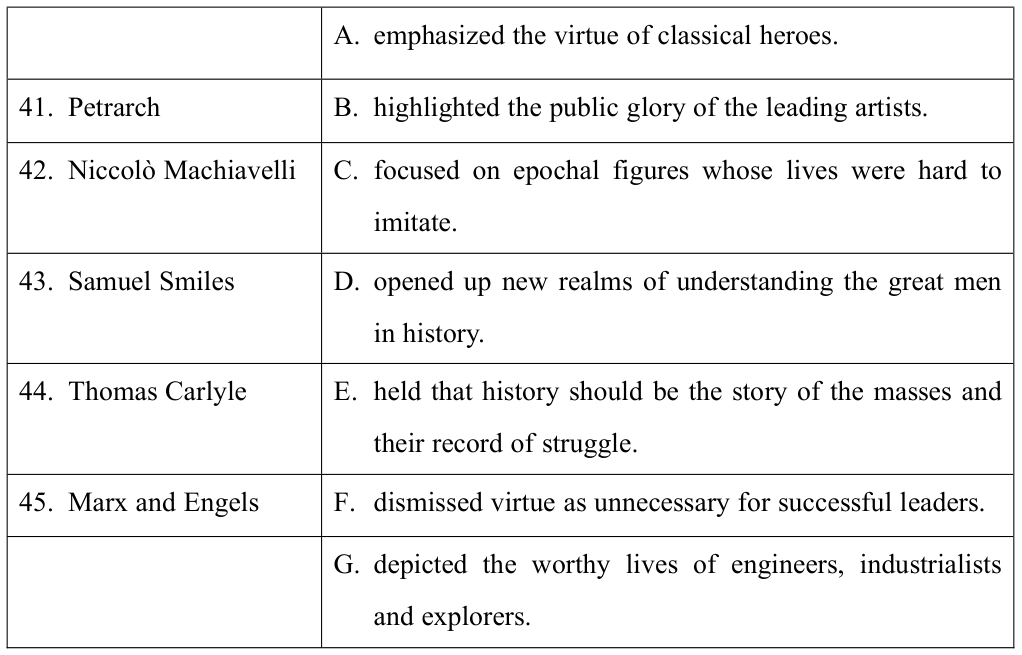
\includegraphics[width=.85\linewidth,height=.55\textheight,keepaspectratio]{2012-02.assets/figure-012-003.png}\end{center}

\subsection*{\textbf{Section III Translation}}


\textbf{46. Directions:}


Translate the following text from English into Chinese. Write your translation on the ANSWER SHEET. (15 points)


When people in developing countries worry about migration, they are usually concerned at the prospect of their best and brightest departure to Silicon Valley or to hospitals and universities in the developed world. These are the kind of workers that countries like Britain, Canada and Australia try to attract by using immigration rules that privilege college graduates.


Lots of studies have found that well-educated people from developing countries are particularly likely to emigrate. A big survey of Indian households in 2004 found that nearly 40\% of emigrants had more than a high-school education, compared with around


3.3\% of all Indians over the age of 25. This “brain drain” has long bothered policymakers in poor countries. They fear that it hurts their economies, depriving them of much-needed skilled workers who could have taught at their universities, worked in their hospitals and come up with clever new products for their factories to make.


\subsection*{\textbf{Section IV Writing}}


\subsection*{\textbf{Part A}}


\textbf{47. Directions:}


Suppose you have found something wrong with the electronic dictionary that you bought from an online store the other day. Write an email to the customer service center to


1) make a complaint, and


2) demand a prompt solution.


You should write about 100 words on the ANSWER SHEET.


\textbf{Do not }sign your own name at the end of the letter. Use “Zhang Wei” instead.


\textbf{Do not} write the address. (10 points)


\subsection*{\textbf{Part B}}


\textbf{48. Directions:}


Write an essay based on the following table. In your writing, you should


\textbf{1) describe the table, and}


\textbf{2) give your comments.}


You should write at least 150 words.


Write your essay on the ANSWER SHEET. (15 points)


\begin{center}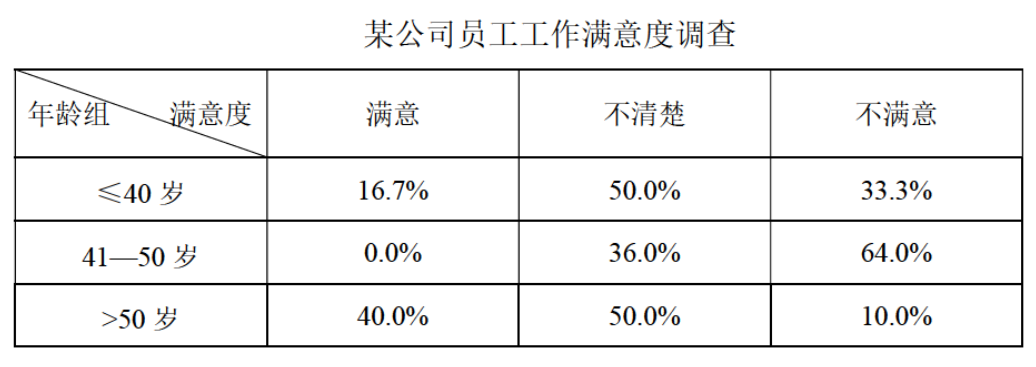
\includegraphics[width=.85\linewidth,height=.55\textheight,keepaspectratio]{2012-02.assets/figure-014-007.png}\end{center}
\end{document}